\documentclass[12pt, twoside]{article}
\input{../preamble}

\fancyhead[LO]{La Scuola d'Italia / Dr.\ Huson / IB Math: Quiz \\* 13 March 2026}
\fancyhead[RO]{\fbox{\begin{minipage}{4cm}\footnotesize First \& Last name:\\[0.5cm]\end{minipage}}}
\fancyfoot[C]{\thepage}

\begin{document}
\subsubsection*{4.19 Quiz: Normal and Binomial Distribution}

\begin{enumerate}[itemsep=0.15cm]

%--- Problem 1: Simple Binomial ---
\item A market stall sells bags of apples. It is known that 20\% of the apples
      have bruises. A bag contains 10 randomly selected apples.
      Let $X$ be the number of bruised apples in the bag.

\begin{center}
\vspace{-0.3cm}
\begin{tikzpicture}[scale=0.55]
  \draw[-{Stealth}] (-0.8,0) -- (7,0) node[right] {$x$};
  \draw[-{Stealth}] (0,-0.5) -- (0,4.5) node[above] {$\mathrm{P}(X=x)$};
  \foreach \x/\h in {0/1.07, 1/2.68, 2/3.02, 3/2.01, 4/0.88, 5/0.26} {
    \fill[gray!30] (\x-0.35,0) rectangle (\x+0.35,\h);
    \draw (\x-0.35,0) rectangle (\x+0.35,\h);
  }
  \foreach \x in {0,...,5} \draw (\x,0.1)--(\x,-0.1) node[below]{\small\x};
  \foreach \y/\l in {1/0.1, 2/0.2, 3/0.3}
    {\draw (0.1,\y)--(-0.1,\y) node[left]{\small\l};}
\end{tikzpicture}
\vspace{-0.3cm}
\end{center}

\begin{enumerate}[itemsep=0.1cm]
  \item Find the expected number of bruised apples in a bag, $E(X)$. \hfill [1]
  \item Find the probability that none of the apples are bruised. \hfill [2]
  \item Find $\mathrm{P}(X = 3)$. \hfill [2]
  \item Find $\mathrm{P}(X \leq 3)$. \hfill [2]
\end{enumerate}

\begin{tikzpicture}
  \draw (-0.6,0) rectangle (11,10);
  \foreach \y in {1,2,3,4,5,6,7,8,9,10} \draw[dotted] (0,\y)--(10.5,\y);
\end{tikzpicture}

\newpage

%--- Problem 2: Simple Normal ---
\item The marks on a mathematics test follow a normal distribution
      with mean $\mu = 72$ and standard deviation $\sigma = 8$.

\begin{center}
\vspace{-0.3cm}
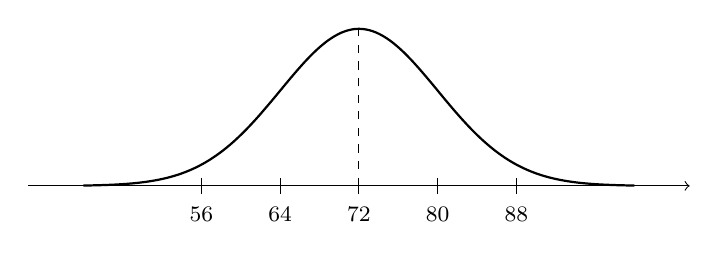
\begin{tikzpicture}[xscale=1, yscale=5]
  \draw[->] (-4.2,0) -- (4.2,0);
  \draw[thick, smooth, domain=-3.5:3.5, samples=80]
    plot (\x, {exp(-0.5*\x*\x)/2.507});
  \draw[dashed] (0,0) -- (0,0.399);
  \foreach \v/\l in {-2/56, -1/64, 0/72, 1/80, 2/88}
    {\draw (\v,0.02)--(\v,-0.02); \node[below] at (\v,-0.03) {\footnotesize\l};}
\end{tikzpicture}
\vspace{-0.3cm}
\end{center}

\begin{enumerate}[itemsep=0.1cm]
  \item Find the probability that a randomly selected student scores
        higher than 85. \hfill [2]
  \item Find the probability that a student's mark is between
        60 and 80. \hfill [2]
  \item 75\% of the students score less than $h$ marks. Find $h$. \hfill [3]
\end{enumerate}

\begin{tikzpicture}
  \draw (-0.6,0) rectangle (11,8);
  \foreach \y in {1,2,3,4,5,6,7} \draw[dotted] (0,\y)--(10.5,\y);
\end{tikzpicture}

\subsubsection*{Answer this section on a separate piece of lined paper}

%--- Problem 3: Combined Normal + Binomial ---
\item The waiting time $T$ (minutes) at a bus stop follows a normal
      distribution with mean 15 minutes and standard deviation $\sigma$ minutes.
      It is known that 4\% of waits are longer than 20 minutes.

\begin{enumerate}[itemsep=0.2cm]
  \item Find the value of $\sigma$. \hfill [3]
  \item Find $\mathrm{P}(T < 12)$. \hfill [2]
  \item On a particular day, 10 people wait at this bus stop. Find the probability \\that
        at most 2 of them wait more than 20 minutes. \hfill [3]
  \item A person is selected at random. Given that they waited less than
        15 minutes, \\find the probability that they waited less than
        10 minutes. \hfill [3]
\end{enumerate}


\end{enumerate}
\end{document}

Solutions
  Problem 1 — Binomial, X ~ B(10, 0.20):
  - (a) E(X) = 10 × 0.20 = 2
  - (b) P(X=0) = 0.80^10 = 0.10737... ≈ 0.107
  - (c) P(X=2) = binomPdf(10, 0.20, 2) = 0.30199... ≈ 0.302
  - (d) P(X≤1) = binomCdf(10, 0.20, 0, 1) = 0.37581... ≈ 0.376

  Problem 2 — Normal, M ~ N(72, 8²):
  - (a) P(M > 85) = normCdf(85, 1E99, 72, 8) = 0.05208... ≈ 0.0521
  - (b) P(60 < M < 80) = normCdf(60, 80, 72, 8) = 0.77453... ≈ 0.775
  - (c) h = invNorm(0.75, 72, 8) = 77.396... ≈ 77.4

  Problem 3 — Combined Normal + Binomial, T ~ N(12, σ²):
  - (a) P(T > 20) = 0.04: invNorm(0.96) = 1.7507; σ = 8/1.7507 = 4.570... ≈ 4.57
  - (b) P(T < 6) = normCdf(0, 6, 12, 4.570) = 0.09459... ≈ 0.0946
  - (c) Y ~ B(18, 0.0946): P(Y ≤ 2) = binomCdf(18, 0.0946, 0, 2) = 0.7659... ≈ 0.766
  - (d) P(T<6|T<15) = P(T<6)/P(T<15) = 0.0946/normCdf(0,15,12,4.570) = 0.0946/0.7443 = 0.1271... ≈ 0.127
